\documentclass{article}

\usepackage{microtype}
\usepackage{graphicx}
\usepackage{float}

\title{Performance and Simulation of Social Networks}
\author{Jakob Wyatt\\19477143}

\begin{document}
\maketitle
\section{Abstract}
\pagebreak
\section{Background}
This report focuses on simulating simple social media networks,
and evaluates the effectiveness of a network given parameters
of that network.\\
The social network consists of a set of users that may follow eachother,
which has been represented in code as a directed graph. Users may not follow themselves,
or follow eachother more than once.\\
There exists only one post at a time, with a new post being loaded when the current
post has not had any activity in the last timestep. The original poster always
likes their own post. A user can only like a post once.\\
The simulation consists
of timesteps, with a function \texttt{update()} to move between timesteps.
The update algorithm works as follows:
\begin{enumerate}
    \item Check that there exists some users that have liked the post in the previous timestep.
            If there are none, the update ends and the next post is loaded.
    \item Iterate through all users who liked the post in the previous timestep.
            Each of their followers is 'exposed' to the post, and have a chance of liking the post.
            This chance is sampled from a Bernoulli distribution with probability
            $\mathit{clamp}\left(\mathit{prob\_like} \times \mathit{clickbait\_factor}, 0, 1\right)$.
    \item If a user likes a post in the current timestep, they have a chance of following the
            original poster. This is sampled using the same technique as above, with global probability
            $\mathit{prob\_foll}$.
\end{enumerate}
Note that in the above algorithm, if a user does not like a post, they may potentially
be exposed to it later via a different friend. This behaviour is intentional, as it incentivises
a highly connected network.

Some parameters that will be varied in the creation of the social network include:
\begin{itemize}
    \item Probability of liking a post
    \item Probability of following a user
    \item Number of users
\end{itemize}

Some parameters that will be tracked throughout the simulation include:
\begin{itemize}
    \item Clustering Coefficient
    \item Average and s.d. of followers per user
    \item Likes per user per post
\end{itemize}

\section{Methodology}

Terminology in this section includes the word 'predecessor' and 'successor'
in the context of graphs. If there is a directed edge between verticies
$A \rightarrow B$, then B is a successor of A and A is a predecessor of B.

\subsection{Parameter Gridsearch}

To profile multiple runs of the simulation a gridsearch algorithm was used
to vary the below parameters:
\begin{itemize}
\item Average and s.d. of followers per user
\item Like/Follow probabilities
\item Number of users in the network
\end{itemize}

First, arrays that contain the parameter values to be tested were created.
Next, for all possible combinations of these parameters, a network
matching these parameters was created. A simulation was then run on all networks,
with simulation statistics being logged to a file as CSV data.

Parameters that are varied in this function are the like and follow probabilities,
network size, clickbait standard deviation, post/timestep number, and
follower average (density) / follower standard deviation (relative popularity).

An advantage of this algorithm is that it is very easy to implement compared to
other search space algorithms, such as gradient descent and evolution.
However, a disadvantage is that it searches a very large volume when the parameter
space has many dimensions (curse of dimensionality), causing a large amount of
time to generate the data. The algorithmic complexity of the gridsearch algorithm
is $O(x^n)$, where n is the number of parameters that are varied and x is the number
of datapoints per parameter.

\subsection{Statistics}
Throughout the simulation, various statistics about the state of the network were
computed. These included the average/s.d. followers per user and the average number of likes
per user.
One particularly interesting statistic that was calculated was the Clustering Coefficient.
To calculate the clustering coefficient of a vertex $V$, the neighbourhood of that
vertex is first found.\\
$N = V_{successors} \bigcup V_{predecessors}$\\
Next, the number of connections between nodes in this neighbourhood is found.\\
$C = |{e_{jk} : v_j, v_j \in N, e_{jk} \in E}|$\\
Finally, this is divided by the total number of potential connections within the neighbourhood.\\
$\mathit{Clustering Coefficient} = \frac{C}{|N| \times (|N| - 1)}$\\
To find the network average clustering coefficient, the clustering coefficient
is calculated for all verticies in the network and averaged.
As the number of followers will always increase over time in this simulation,
to enable comparison between clustering coefficients at different timesteps,
the network average clustering coefficient was then divided by the number
of edges in the graph.
This algorithm has $O\left(n^3\right)$ execution time when hashtables are used to store
edges and verticies, which is done in this program.
When a linked list is used instead, this execution time degrades to $O\left(n^4\right)$.

\subsection{Graph Generation}

To generate the simulated networks, a unique algorithm was used
that was created by the author, and to their knowledge, does not exist anywhere else.
This algorithm allows efficient generation of structured (non-random) networks,
with a consistent runtime complexity of $O\left(V \times E\right)$.

First, a number of verticies are created.
Next, these verticies are iterated over, and the number of successors of each
vertex is calculated by sampling from a distribution $X \sim N\left(follower\_av, follwer\_sd^2\right)$.

To select the edges of the network, an approach was used that is similar in concept
to a variogram, used in the field of geostatistics.
A variogram measures the amount of correlation between two points that are some distance apart.
In this algorithm, this distance is discrete rather than continuous, and is measured by finding
some path between two nodes. By increasing the spacial correlation at short distances,
a graph can be created with a higher clustering coefficient. Reducing the spacial correlation
to 0 causes the graph to become random.

A property of a graph that is analogous to the variogram is the clustering
coefficient, which determines the correlation between verticies at a distance of 1.
This clustering coefficient can be generalized to include all verticies
within some distance $h$ of a central vertex (Xiao et al. 2007).
It is expected that this clustering coefficient will decrease as the distance increases
in a real life network. An example of this is that your friends are likely to be friends of
eachother, but your friends of friends are less likely to be friends of eachother.
By assuming the correlation between verticies, realistic social networks can be generated
for testing.

To generate an edge in the graph, a random walk is performed starting at a given vertex, $V_0$.
This random walk occurs along any nodes that are predecessors of the current node,
and does not loop back onto previously visited nodes.
At each step on the random walk, the probability of creating an edge with $V_0$
is calculated by evaluating the variogram using the distance from the original node
(length of the random walk).
If an edge is created, the process
starts again and repeats until all necessary edges have been created.
If there are no available verticies to walk to,
or the random walk has reached some distance threshold from the original node,
an edge is created with any random vertex in the graph. This allows initial
'bootstrapping' of the network when no edges have yet been created.

\subsection{Time and Space Complexity}
The post propogation algorithm used in this program has a time complexity of
$O\left(V \times E\right)$. However, many algorithms that calculate statistics about the network have a much
worse time complexity. One example is the calculation of the clustering coefficient,
which has a time complexity of $O\left(V^3\right)$ when implemented using a hash table
and $O\left(V^4\right)$ when implemented using a linked list.
The space complexity of this program is $O\left(V + E\right)$. Although
a large amount of caching is used to speed up the program, none of this caching
is non-linear in the size of the input data.

\subsection{Execution}
The generated data for this simulation can be found in report/data.csv.
This data can be created by running the program found in src/SocialNetworkSimRunner.py.
This program takes approximately 30 minutes to run on an i7-7700k processor.
Gridsearch parameters can be changed within the gridsearch function.

\section{Results}

It was found that clustering coefficient did not change significantly over the
course of the simulation, and either increases or decreases by a maximum of 10\%.
This suggests that over time, friend groups within the network do not increase
or decrease the amount of connections within the group, relative to all other connections.

Follower average per person, as well as likes per person, all increased over time.
This was expected, as there is no mechanism for unliking or unfollowing a user
within the simulation mode, and post. The rate of change also increased over time;
however, this behaviour could only be observed when the like and follow probabilities
were low. With a high probability, such as 0.5, posts often 'saturate' the network,
and give data that is not representative of a real life situation.
\begin{figure}[H]
\centering
\begin{minipage}{.5\textwidth}
  \centering
  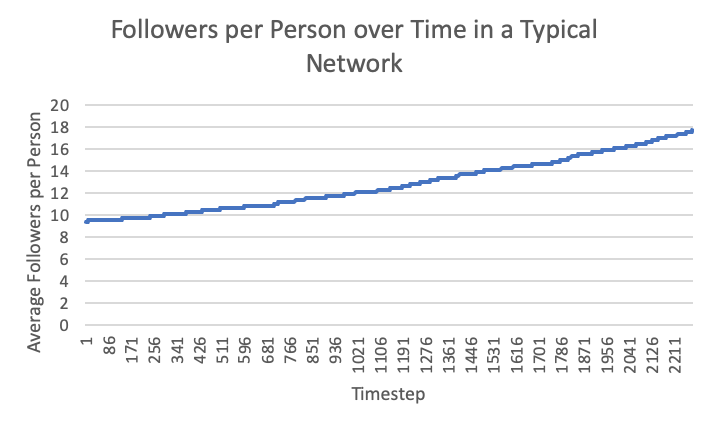
\includegraphics[width=\linewidth]{follAv}
\end{minipage}\hfill
\begin{minipage}{.5\textwidth}
  \centering
  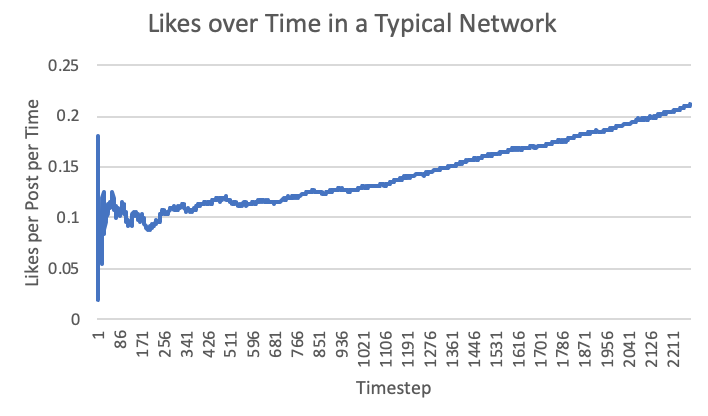
\includegraphics[width=\linewidth]{likes}
\end{minipage}
\end{figure}

Follower s.d. per person also increased over time. However, when scaled with respect
to the total number of followers, it was observed to decrease over time,
eventually reaching a stable value. For networks with initial s.d. = 0,
the follower s.d. per person would quickly rise to a low, stable value.
Follower s.d. is analagous to fame within a network - the higher the s.d,
the more people have very high or very low follower counts.
This result shows that fame within a network generally decreases over time,
and is a result of the network eventually reaching a state of equilibrium.

When the standard deviation of the clickbait factor was increased, the standard
deviation of the followers per person was also seen to increase over time.
This shows that use of clickbait, within this simulation, is an effective
tool to gain fame within the network.
However, when the s.d. of the clickbait factor is further increased,
the s.d. of followers per person only increases by a small amount.
This demonstrates the law of diminishing returns.

\begin{figure}[H]
\centering
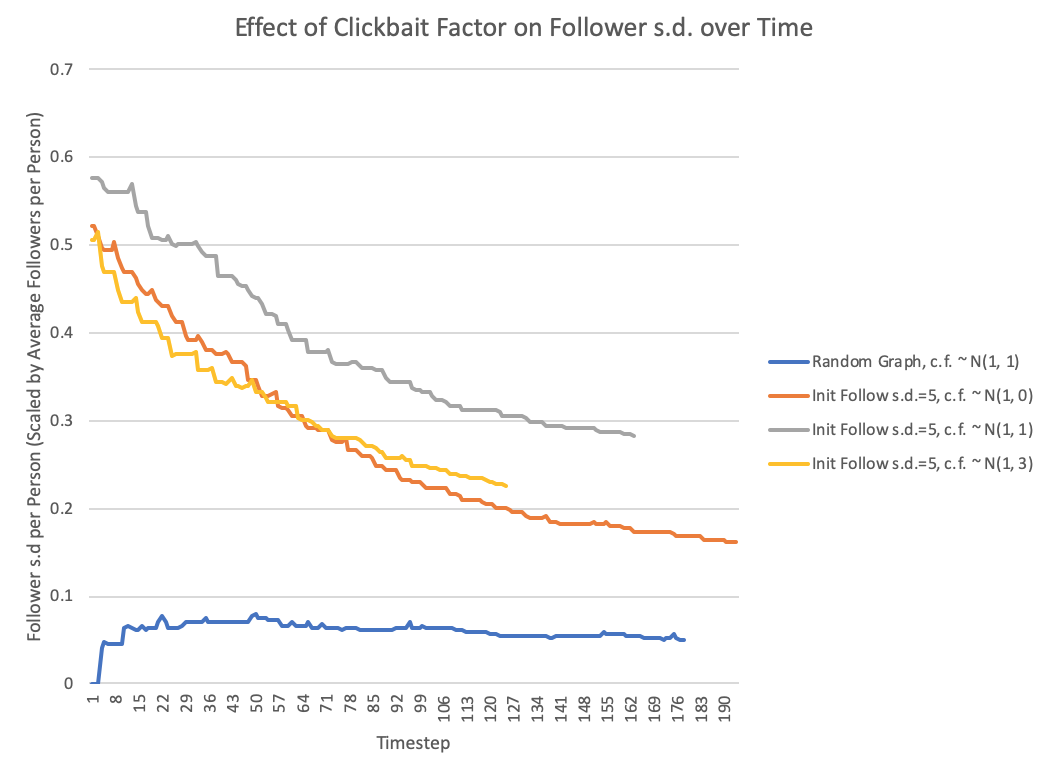
\includegraphics[width=\linewidth]{follSd}
\end{figure}

Another question that can be asked about a social network is
the tradeoff between the like probability and the follow probability.
If the follow probability is low, the user base will stagnate and there will
not be as much growth on posts.
In contrast, if the like probability is low, the company will find it difficult
to make money. What is the best tradeoff between these two options?

It can be seen from the above graphs that despite having a higher initial
proportion of likes, the blue network stagnates and does not grow. Because of this,
it is eventually beat by the second network, which started out with a lower proportion
of likes, but had a higher probability of following the user.
This shows that when creating a social network, content that is relevant
to the user may help to grow the platform long term. By only showing
sensationalist non-personalized content to the user, they may be less likely to follow the original poster.
This causes stagnation and a lack of growth within a network.

\begin{figure}[H]
\centering
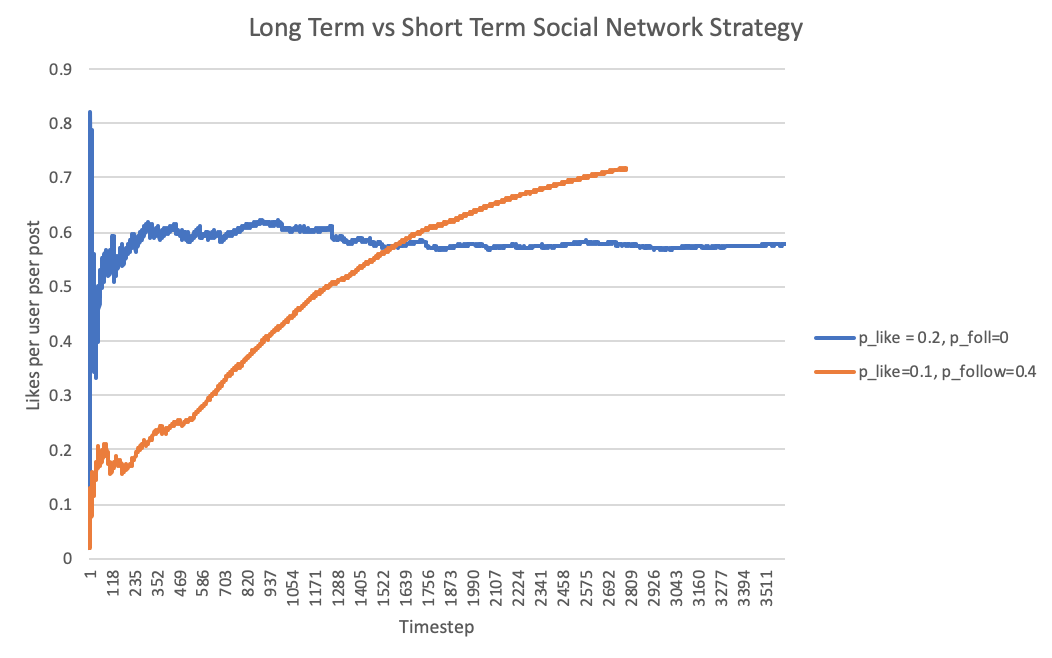
\includegraphics[width=\linewidth]{Growth}
\end{figure}

\section{Conclusion and Future Work}
Despite being simple, the social network model and algorithm that was used
in this assignment was still able to exhibit many of the properties
that would be expected in a social network, such as friend grouping,
fame, clickbait, and personalized content.
One application of social network simulations could be to predict the outcome
of a social network policy change before it is deployed.
Another application of this simulation could be to model spread of disease, to evaluate the effectiveness
of different methods to block the disease.

Future work that could be done on this simulation involve both better
analysis of the current data, generation of networks using different algorithms,
and implementing more graph statistics to measure.

Due to time constraints, only a limited amount of basic analysis could be done
on generated data. This analysis was mostly constrained to setting constant values for certain
parameters, and varying a single parameter at a time to see the outcome.
This assumes that each parameter is independent, however this may not be the case.

A more in-depth analysis could involve principal component analysis to rigorously
determine the most important factors in the performance of a social network.

The current algorithm used to generate random graphs with structure is not mathematically rigorous.
One method of verifying the results of this algorithm would be to implement a different
graph generation algorithm such as ClustRNet (Bansal, Khandelwal, and Meyers, 2009),
and compare the results with the current method of generating random graphs.
This was not done due to time constraints.

Only a small amount of statistics related to graphs were analysed. To improve this
analysis in future, a wider range of statistics about the graph could be calculated at each time step,
including but not limited to:
\begin{itemize}
\item Mutuality (The probability that someone is followed back)
\item Distance (The minimum number of edges required to connect any two verticies in the graph)
\item Centrality of highly followed users (How much influence does a node have)
\end{itemize}
This would allow a more in depth analysis into the factors behind social network performance, and a better
comparison with real life networks.

More work that could be done to improve this simulation would be to increase
its complexity. One possible way of doing this could be to introduce
individual like probabilities per user. However,
this added complexity would not be worth the implementation time required,
with the previous three suggestions offering greater benefit for less development
time.

\section{References}
Xiao, Wenjun, Wenhong Wei, Weidong Chen, Yong Qin, Behrooz Parhami. 2007.
\textit{Extended Clustering Coefficients: Generalization of Clustering Coefficients in Small-World
Networks}. Journal of Systems Science and Systems Engineering. https://www.ece.ucsb.edu/~parhami/pubs\_folder/parh07-jssse-ext-clustering-coeff.pdf\\

Bansal, Shweta, Shashank Khandelwal, and Lauren Ancel Meyers. 2009. \textit{Exploring Biological Network Structure with Clustered Random Networks}.
BMC Bioinformatics. https://bmcbioinformatics.biomedcentral.com/articles/10.1186/1471-2105-10-405



\end{document}
